\documentclass[1p]{elsarticle_modified}
%\bibliographystyle{elsarticle-num}

%\usepackage[colorlinks]{hyperref}
%\usepackage{abbrmath_seonhwa} %\Abb, \Ascr, \Acal ,\Abf, \Afrak
\usepackage{amsfonts}
\usepackage{amssymb}
\usepackage{amsmath}
\usepackage{amsthm}
\usepackage{scalefnt}
\usepackage{amsbsy}
\usepackage{kotex}
\usepackage{caption}
\usepackage{subfig}
\usepackage{color}
\usepackage{graphicx}
\usepackage{xcolor} %% white, black, red, green, blue, cyan, magenta, yellow
\usepackage{float}
\usepackage{setspace}
\usepackage{hyperref}

\usepackage{tikz}
\usetikzlibrary{arrows}

\usepackage{multirow}
\usepackage{array} % fixed length table
\usepackage{hhline}

%%%%%%%%%%%%%%%%%%%%%
\makeatletter
\renewcommand*\env@matrix[1][\arraystretch]{%
	\edef\arraystretch{#1}%
	\hskip -\arraycolsep
	\let\@ifnextchar\new@ifnextchar
	\array{*\c@MaxMatrixCols c}}
\makeatother %https://tex.stackexchange.com/questions/14071/how-can-i-increase-the-line-spacing-in-a-matrix
%%%%%%%%%%%%%%%

\usepackage[normalem]{ulem}

\newcommand{\msout}[1]{\ifmmode\text{\sout{\ensuremath{#1}}}\else\sout{#1}\fi}
%SOURCE: \msout is \stkout macro in https://tex.stackexchange.com/questions/20609/strikeout-in-math-mode

\newcommand{\cancel}[1]{
	\ifmmode
	{\color{red}\msout{#1}}
	\else
	{\color{red}\sout{#1}}
	\fi
}

\newcommand{\add}[1]{
	{\color{blue}\uwave{#1}}
}

\newcommand{\replace}[2]{
	\ifmmode
	{\color{red}\msout{#1}}{\color{blue}\uwave{#2}}
	\else
	{\color{red}\sout{#1}}{\color{blue}\uwave{#2}}
	\fi
}

\newcommand{\Sol}{\mathcal{S}} %segment
\newcommand{\D}{D} %diagram
\newcommand{\A}{\mathcal{A}} %arc


%%%%%%%%%%%%%%%%%%%%%%%%%%%%%5 test

\def\sl{\operatorname{\textup{SL}}(2,\Cbb)}
\def\psl{\operatorname{\textup{PSL}}(2,\Cbb)}
\def\quan{\mkern 1mu \triangleright \mkern 1mu}

\theoremstyle{definition}
\newtheorem{thm}{Theorem}[section]
\newtheorem{prop}[thm]{Proposition}
\newtheorem{lem}[thm]{Lemma}
\newtheorem{ques}[thm]{Question}
\newtheorem{cor}[thm]{Corollary}
\newtheorem{defn}[thm]{Definition}
\newtheorem{exam}[thm]{Example}
\newtheorem{rmk}[thm]{Remark}
\newtheorem{alg}[thm]{Algorithm}

\newcommand{\I}{\sqrt{-1}}
\begin{document}

%\begin{frontmatter}
%
%\title{Boundary parabolic representations of knots up to 8 crossings}
%
%%% Group authors per affiliation:
%\author{Yunhi Cho} 
%\address{Department of Mathematics, University of Seoul, Seoul, Korea}
%\ead{yhcho@uos.ac.kr}
%
%
%\author{Seonhwa Kim} %\fnref{s_kim}}
%\address{Center for Geometry and Physics, Institute for Basic Science, Pohang, 37673, Korea}
%\ead{ryeona17@ibs.re.kr}
%
%\author{Hyuk Kim}
%\address{Department of Mathematical Sciences, Seoul National University, Seoul 08826, Korea}
%\ead{hyukkim@snu.ac.kr}
%
%\author{Seokbeom Yoon}
%\address{Department of Mathematical Sciences, Seoul National University, Seoul, 08826,  Korea}
%\ead{sbyoon15@snu.ac.kr}
%
%\begin{abstract}
%We find all boundary parabolic representation of knots up to 8 crossings.
%
%\end{abstract}
%\begin{keyword}
%    \MSC[2010] 57M25 
%\end{keyword}
%
%\end{frontmatter}

%\linenumbers
%\tableofcontents
%
\newcommand\colored[1]{\textcolor{white}{\rule[-0.35ex]{0.8em}{1.4ex}}\kern-0.8em\color{red} #1}%
%\newcommand\colored[1]{\textcolor{white}{ #1}\kern-2.17ex	\textcolor{white}{ #1}\kern-1.81ex	\textcolor{white}{ #1}\kern-2.15ex\color{red}#1	}

{\Large $\underline{12n_{0078}~(K12n_{0078})}$}

\setlength{\tabcolsep}{10pt}
\renewcommand{\arraystretch}{1.6}
\vspace{1cm}\begin{tabular}{m{100pt}>{\centering\arraybackslash}m{274pt}}
\multirow{5}{120pt}{
	\centering
	\includegraphics[width=112pt]{../../../GIT/diagram.site/Diagrams/png/2167_12n_0078.png}\\
\ \ \ A knot diagram\footnotemark}&
\allowdisplaybreaks
\textbf{Linearized knot diagam} \\
\cline{2-2}
 &
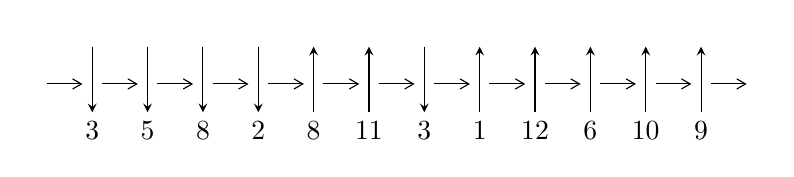
\begin{tikzpicture}[x=20pt, y=17pt]
	% nodes
	\node (C0) at (0, 0) {};
	\node (C1) at (1, 0) {};
	\node (C1U) at (1, +1) {};
	\node (C1D) at (1, -1) {3};

	\node (C2) at (2, 0) {};
	\node (C2U) at (2, +1) {};
	\node (C2D) at (2, -1) {5};

	\node (C3) at (3, 0) {};
	\node (C3U) at (3, +1) {};
	\node (C3D) at (3, -1) {8};

	\node (C4) at (4, 0) {};
	\node (C4U) at (4, +1) {};
	\node (C4D) at (4, -1) {2};

	\node (C5) at (5, 0) {};
	\node (C5U) at (5, +1) {};
	\node (C5D) at (5, -1) {8};

	\node (C6) at (6, 0) {};
	\node (C6U) at (6, +1) {};
	\node (C6D) at (6, -1) {11};

	\node (C7) at (7, 0) {};
	\node (C7U) at (7, +1) {};
	\node (C7D) at (7, -1) {3};

	\node (C8) at (8, 0) {};
	\node (C8U) at (8, +1) {};
	\node (C8D) at (8, -1) {1};

	\node (C9) at (9, 0) {};
	\node (C9U) at (9, +1) {};
	\node (C9D) at (9, -1) {12};

	\node (C10) at (10, 0) {};
	\node (C10U) at (10, +1) {};
	\node (C10D) at (10, -1) {6};

	\node (C11) at (11, 0) {};
	\node (C11U) at (11, +1) {};
	\node (C11D) at (11, -1) {10};

	\node (C12) at (12, 0) {};
	\node (C12U) at (12, +1) {};
	\node (C12D) at (12, -1) {9};
	\node (C13) at (13, 0) {};

	% arrows
	\draw[->,>={angle 60}]
	(C0) edge (C1) (C1) edge (C2) (C2) edge (C3) (C3) edge (C4) (C4) edge (C5) (C5) edge (C6) (C6) edge (C7) (C7) edge (C8) (C8) edge (C9) (C9) edge (C10) (C10) edge (C11) (C11) edge (C12) (C12) edge (C13) ;	\draw[->,>=stealth]
	(C1U) edge (C1D) (C2U) edge (C2D) (C3U) edge (C3D) (C4U) edge (C4D) (C5D) edge (C5U) (C6D) edge (C6U) (C7U) edge (C7D) (C8D) edge (C8U) (C9D) edge (C9U) (C10D) edge (C10U) (C11D) edge (C11U) (C12D) edge (C12U) ;
	\end{tikzpicture} \\
\hhline{~~} \\& 
\textbf{Solving Sequence} \\ \cline{2-2} 
 &
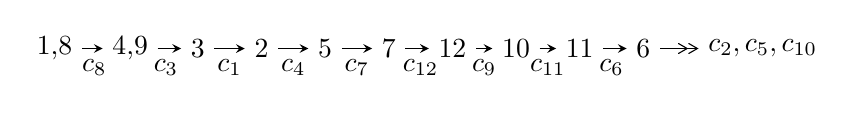
\begin{tikzpicture}[x=23pt, y=7pt]
	% node
	\node (A0) at (-1/8, 0) {1,8};
	\node (A1) at (17/16, 0) {4,9};
	\node (A2) at (17/8, 0) {3};
	\node (A3) at (25/8, 0) {2};
	\node (A4) at (33/8, 0) {5};
	\node (A5) at (41/8, 0) {7};
	\node (A6) at (49/8, 0) {12};
	\node (A7) at (57/8, 0) {10};
	\node (A8) at (65/8, 0) {11};
	\node (A9) at (73/8, 0) {6};
	\node (C1) at (1/2, -1) {$c_{8}$};
	\node (C2) at (13/8, -1) {$c_{3}$};
	\node (C3) at (21/8, -1) {$c_{1}$};
	\node (C4) at (29/8, -1) {$c_{4}$};
	\node (C5) at (37/8, -1) {$c_{7}$};
	\node (C6) at (45/8, -1) {$c_{12}$};
	\node (C7) at (53/8, -1) {$c_{9}$};
	\node (C8) at (61/8, -1) {$c_{11}$};
	\node (C9) at (69/8, -1) {$c_{6}$};
	\node (A10) at (11, 0) {$c_{2},c_{5},c_{10}$};

	% edge
	\draw[->,>=stealth]	
	(A0) edge (A1) (A1) edge (A2) (A2) edge (A3) (A3) edge (A4) (A4) edge (A5) (A5) edge (A6) (A6) edge (A7) (A7) edge (A8) (A8) edge (A9) ;
	\draw[->>,>={angle 60}]	
	(A9) edge (A10);
\end{tikzpicture} \\ 

\end{tabular} \\

\footnotetext{
The image of knot diagram is generated by the software ``\textbf{Draw programme}" developed by Andrew Bartholomew(\url{http://www.layer8.co.uk/maths/draw/index.htm\#Running-draw}), where we modified some parts for our purpose(\url{https://github.com/CATsTAILs/LinksPainter}).
}\phantom \\ \newline 
\centering \textbf{Ideals for irreducible components\footnotemark of $X_{\text{par}}$} 
 
\begin{align*}
I^u_{1}&=\langle 
37387481608 u^{36}-262071379227 u^{35}+\cdots+62312469363 b+37745018210,\\
\phantom{I^u_{1}}&\phantom{= \langle  }39879980401 u^{36}-353616847554 u^{35}+\cdots+62312469363 a+919059301277,\\
\phantom{I^u_{1}}&\phantom{= \langle  }u^{37}-8 u^{36}+\cdots+19 u-1\rangle \\
I^u_{2}&=\langle 
b,\;- u^4- u^3-4 u^2+a-3 u-3,\;u^5+u^4+4 u^3+3 u^2+3 u+1\rangle \\
\\
\end{align*}
\raggedright * 2 irreducible components of $\dim_{\mathbb{C}}=0$, with total 42 representations.\\
\footnotetext{All coefficients of polynomials are rational numbers. But the coefficients are sometimes approximated in decimal forms when there is not enough margin.}
\newpage
\renewcommand{\arraystretch}{1}
\centering \section*{I. $I^u_{1}= \langle 3.74\times10^{10} u^{36}-2.62\times10^{11} u^{35}+\cdots+6.23\times10^{10} b+3.77\times10^{10},\;3.99\times10^{10} u^{36}-3.54\times10^{11} u^{35}+\cdots+6.23\times10^{10} a+9.19\times10^{11},\;u^{37}-8 u^{36}+\cdots+19 u-1 \rangle$}
\flushleft \textbf{(i) Arc colorings}\\
\begin{tabular}{m{7pt} m{180pt} m{7pt} m{180pt} }
\flushright $a_{1}=$&$\begin{pmatrix}0\\u\end{pmatrix}$ \\
\flushright $a_{8}=$&$\begin{pmatrix}1\\0\end{pmatrix}$ \\
\flushright $a_{4}=$&$\begin{pmatrix}-0.640000 u^{36}+5.67490 u^{35}+\cdots+118.964 u-14.7492\\-0.600000 u^{36}+4.20576 u^{35}+\cdots+2.58902 u-0.605738\end{pmatrix}$ \\
\flushright $a_{9}=$&$\begin{pmatrix}1\\- u^2\end{pmatrix}$ \\
\flushright $a_{3}=$&$\begin{pmatrix}-1.24000 u^{36}+9.88066 u^{35}+\cdots+121.553 u-15.3549\\-0.600000 u^{36}+4.20576 u^{35}+\cdots+2.58902 u-0.605738\end{pmatrix}$ \\
\flushright $a_{2}=$&$\begin{pmatrix}-0.440000 u^{36}+4.28395 u^{35}+\cdots+104.318 u-12.1296\\-0.400000 u^{36}+2.79424 u^{35}+\cdots+2.41098 u-0.394262\end{pmatrix}$ \\
\flushright $a_{5}=$&$\begin{pmatrix}-0.600000 u^{36}+4.20165 u^{35}+\cdots+21.8826 u-3.88735\\-0.400000 u^{36}+2.79424 u^{35}+\cdots+2.41098 u-0.394262\end{pmatrix}$ \\
\flushright $a_{7}=$&$\begin{pmatrix}-0.394262 u^{36}+2.75410 u^{35}+\cdots+35.8645 u-5.08000\\-0.598354 u^{36}+4.78683 u^{35}+\cdots+7.51265 u-0.600000\end{pmatrix}$ \\
\flushright $a_{12}=$&$\begin{pmatrix}- u\\u^3+u\end{pmatrix}$ \\
\flushright $a_{10}=$&$\begin{pmatrix}u^2+1\\- u^4-2 u^2\end{pmatrix}$ \\
\flushright $a_{11}=$&$\begin{pmatrix}- u^3-2 u\\u^5+3 u^3+u\end{pmatrix}$ \\
\flushright $a_{6}=$&$\begin{pmatrix}-1.00000 u^{36}+6.99588 u^{35}+\cdots+24.2936 u-4.28162\\-0.400000 u^{36}+2.79424 u^{35}+\cdots+2.41098 u-0.394262\end{pmatrix}$\\&\end{tabular}
\flushleft \textbf{(ii) Obstruction class $= -1$}\\~\\
\flushleft \textbf{(iii) Cusp Shapes $= -\frac{126456874109}{20770823121} u^{36}+\frac{325863614327}{6923607707} u^{35}+\cdots+\frac{5835323526623}{20770823121} u-\frac{551008395754}{20770823121}$}\\~\\
\newpage\renewcommand{\arraystretch}{1}
\flushleft \textbf{(iv) u-Polynomials at the component}\newline \\
\begin{tabular}{m{50pt}|m{274pt}}
Crossings & \hspace{64pt}u-Polynomials at each crossing \\
\hline $$\begin{aligned}c_{1}\end{aligned}$$&$\begin{aligned}
&u^{37}+12 u^{36}+\cdots+5 u+1
\end{aligned}$\\
\hline $$\begin{aligned}c_{2},c_{4}\end{aligned}$$&$\begin{aligned}
&u^{37}-6 u^{36}+\cdots-3 u+1
\end{aligned}$\\
\hline $$\begin{aligned}c_{3},c_{7}\end{aligned}$$&$\begin{aligned}
&u^{37}- u^{36}+\cdots+120 u^2+32
\end{aligned}$\\
\hline $$\begin{aligned}c_{5}\end{aligned}$$&$\begin{aligned}
&u^{37}+2 u^{36}+\cdots+3 u+1
\end{aligned}$\\
\hline $$\begin{aligned}c_{6},c_{10}\end{aligned}$$&$\begin{aligned}
&u^{37}+2 u^{36}+\cdots+3 u+1
\end{aligned}$\\
\hline $$\begin{aligned}c_{8},c_{9},c_{11}\\c_{12}\end{aligned}$$&$\begin{aligned}
&u^{37}-8 u^{36}+\cdots+19 u-1
\end{aligned}$\\
\hline
\end{tabular}\\~\\
\newpage\renewcommand{\arraystretch}{1}
\flushleft \textbf{(v) Riley Polynomials at the component}\newline \\
\begin{tabular}{m{50pt}|m{274pt}}
Crossings & \hspace{64pt}Riley Polynomials at each crossing \\
\hline $$\begin{aligned}c_{1}\end{aligned}$$&$\begin{aligned}
&y^{37}+32 y^{36}+\cdots+5 y-1
\end{aligned}$\\
\hline $$\begin{aligned}c_{2},c_{4}\end{aligned}$$&$\begin{aligned}
&y^{37}-12 y^{36}+\cdots+5 y-1
\end{aligned}$\\
\hline $$\begin{aligned}c_{3},c_{7}\end{aligned}$$&$\begin{aligned}
&y^{37}+33 y^{36}+\cdots-7680 y-1024
\end{aligned}$\\
\hline $$\begin{aligned}c_{5}\end{aligned}$$&$\begin{aligned}
&y^{37}-40 y^{36}+\cdots+19 y-1
\end{aligned}$\\
\hline $$\begin{aligned}c_{6},c_{10}\end{aligned}$$&$\begin{aligned}
&y^{37}-8 y^{36}+\cdots+19 y-1
\end{aligned}$\\
\hline $$\begin{aligned}c_{8},c_{9},c_{11}\\c_{12}\end{aligned}$$&$\begin{aligned}
&y^{37}+44 y^{36}+\cdots+99 y-1
\end{aligned}$\\
\hline
\end{tabular}\\~\\
\newpage\flushleft \textbf{(vi) Complex Volumes and Cusp Shapes}
$$\begin{array}{c|c|c}  
\text{Solutions to }I^u_{1}& \I (\text{vol} + \sqrt{-1}CS) & \text{Cusp shape}\\
 \hline 
\begin{aligned}
u &= \phantom{-}0.192278 + 0.981446 I \\
a &= \phantom{-}0.020576 - 0.394070 I \\
b &= \phantom{-}0.028151 + 0.615473 I\end{aligned}
 & -2.37817 + 2.37893 I & \phantom{-}2.00000 - 4.24354 I \\ \hline\begin{aligned}
u &= \phantom{-}0.192278 - 0.981446 I \\
a &= \phantom{-}0.020576 + 0.394070 I \\
b &= \phantom{-}0.028151 - 0.615473 I\end{aligned}
 & -2.37817 - 2.37893 I & \phantom{-}2.00000 + 4.24354 I \\ \hline\begin{aligned}
u &= \phantom{-}0.954498 + 0.071334 I \\
a &= -0.13625 + 3.34385 I \\
b &= \phantom{-}0.22449 - 1.57573 I\end{aligned}
 & \phantom{-}7.67323 + 3.34146 I & \phantom{-}7.54708 - 2.94673 I \\ \hline\begin{aligned}
u &= \phantom{-}0.954498 - 0.071334 I \\
a &= -0.13625 - 3.34385 I \\
b &= \phantom{-}0.22449 + 1.57573 I\end{aligned}
 & \phantom{-}7.67323 - 3.34146 I & \phantom{-}7.54708 + 2.94673 I \\ \hline\begin{aligned}
u &= \phantom{-}0.739019 + 0.820681 I \\
a &= -0.80030 - 2.64862 I \\
b &= -0.02142 + 1.55446 I\end{aligned}
 & \phantom{-}5.46691 + 2.17037 I & \phantom{-0.000000 } 0 \\ \hline\begin{aligned}
u &= \phantom{-}0.739019 - 0.820681 I \\
a &= -0.80030 + 2.64862 I \\
b &= -0.02142 - 1.55446 I\end{aligned}
 & \phantom{-}5.46691 - 2.17037 I & \phantom{-0.000000 } 0 \\ \hline\begin{aligned}
u &= \phantom{-}0.488581 + 0.716463 I \\
a &= -0.400880 + 0.540394 I \\
b &= \phantom{-}0.929621 - 0.055392 I\end{aligned}
 & -0.60086 + 3.42978 I & \phantom{-}1.46957 - 8.06302 I \\ \hline\begin{aligned}
u &= \phantom{-}0.488581 - 0.716463 I \\
a &= -0.400880 - 0.540394 I \\
b &= \phantom{-}0.929621 + 0.055392 I\end{aligned}
 & -0.60086 - 3.42978 I & \phantom{-}1.46957 + 8.06302 I \\ \hline\begin{aligned}
u &= \phantom{-}0.694171 + 0.952511 I \\
a &= \phantom{-}0.57988 + 2.67460 I \\
b &= \phantom{-}0.43869 - 1.52488 I\end{aligned}
 & \phantom{-}4.63566 + 8.76465 I & \phantom{-0.000000 } 0 \\ \hline\begin{aligned}
u &= \phantom{-}0.694171 - 0.952511 I \\
a &= \phantom{-}0.57988 - 2.67460 I \\
b &= \phantom{-}0.43869 + 1.52488 I\end{aligned}
 & \phantom{-}4.63566 - 8.76465 I & \phantom{-0.000000 } 0\\
 \hline 
 \end{array}$$\newpage$$\begin{array}{c|c|c}  
\text{Solutions to }I^u_{1}& \I (\text{vol} + \sqrt{-1}CS) & \text{Cusp shape}\\
 \hline 
\begin{aligned}
u &= \phantom{-}0.301349 + 0.644967 I \\
a &= -0.44045 + 2.61190 I \\
b &= -0.171200 - 0.710425 I\end{aligned}
 & -2.48892 + 1.77260 I & \phantom{-}1.52089 - 2.95783 I \\ \hline\begin{aligned}
u &= \phantom{-}0.301349 - 0.644967 I \\
a &= -0.44045 - 2.61190 I \\
b &= -0.171200 + 0.710425 I\end{aligned}
 & -2.48892 - 1.77260 I & \phantom{-}1.52089 + 2.95783 I \\ \hline\begin{aligned}
u &= -0.337610 + 0.584660 I \\
a &= -1.40228 + 3.03617 I \\
b &= -0.36360 - 1.42665 I\end{aligned}
 & \phantom{-}2.83785 - 4.34213 I & -1.01036 + 2.76263 I \\ \hline\begin{aligned}
u &= -0.337610 - 0.584660 I \\
a &= -1.40228 - 3.03617 I \\
b &= -0.36360 + 1.42665 I\end{aligned}
 & \phantom{-}2.83785 + 4.34213 I & -1.01036 - 2.76263 I \\ \hline\begin{aligned}
u &= \phantom{-}0.530968 + 0.127903 I \\
a &= -0.409091 - 0.456941 I \\
b &= \phantom{-}0.495562 + 0.299085 I\end{aligned}
 & \phantom{-}1.138660 + 0.126784 I & \phantom{-}8.90691 - 0.21757 I \\ \hline\begin{aligned}
u &= \phantom{-}0.530968 - 0.127903 I \\
a &= -0.409091 + 0.456941 I \\
b &= \phantom{-}0.495562 - 0.299085 I\end{aligned}
 & \phantom{-}1.138660 - 0.126784 I & \phantom{-}8.90691 + 0.21757 I \\ \hline\begin{aligned}
u &= -0.361376 + 0.397065 I \\
a &= \phantom{-}1.91674 - 3.19790 I \\
b &= -0.08394 + 1.41819 I\end{aligned}
 & \phantom{-}3.38035 + 1.79092 I & -0.30116 - 2.50097 I \\ \hline\begin{aligned}
u &= -0.361376 - 0.397065 I \\
a &= \phantom{-}1.91674 + 3.19790 I \\
b &= -0.08394 - 1.41819 I\end{aligned}
 & \phantom{-}3.38035 - 1.79092 I & -0.30116 + 2.50097 I \\ \hline\begin{aligned}
u &= -0.05375 + 1.50789 I \\
a &= \phantom{-}0.41135 - 1.87901 I \\
b &= \phantom{-}0.31409 + 1.45132 I\end{aligned}
 & -2.96990 + 0.48951 I & \phantom{-0.000000 } 0 \\ \hline\begin{aligned}
u &= -0.05375 - 1.50789 I \\
a &= \phantom{-}0.41135 + 1.87901 I \\
b &= \phantom{-}0.31409 - 1.45132 I\end{aligned}
 & -2.96990 - 0.48951 I & \phantom{-0.000000 } 0\\
 \hline 
 \end{array}$$\newpage$$\begin{array}{c|c|c}  
\text{Solutions to }I^u_{1}& \I (\text{vol} + \sqrt{-1}CS) & \text{Cusp shape}\\
 \hline 
\begin{aligned}
u &= \phantom{-}0.121575 + 0.445561 I \\
a &= -0.633975 + 0.683934 I \\
b &= -0.744443 + 0.181579 I\end{aligned}
 & -1.49379 + 0.01486 I & -3.88474 - 1.23232 I \\ \hline\begin{aligned}
u &= \phantom{-}0.121575 - 0.445561 I \\
a &= -0.633975 - 0.683934 I \\
b &= -0.744443 - 0.181579 I\end{aligned}
 & -1.49379 - 0.01486 I & -3.88474 + 1.23232 I \\ \hline\begin{aligned}
u &= \phantom{-}0.04039 + 1.56760 I \\
a &= \phantom{-}0.458186 - 0.041159 I \\
b &= -1.179650 + 0.205890 I\end{aligned}
 & -8.59444 + 0.63473 I & \phantom{-0.000000 } 0 \\ \hline\begin{aligned}
u &= \phantom{-}0.04039 - 1.56760 I \\
a &= \phantom{-}0.458186 + 0.041159 I \\
b &= -1.179650 - 0.205890 I\end{aligned}
 & -8.59444 - 0.63473 I & \phantom{-0.000000 } 0 \\ \hline\begin{aligned}
u &= -0.08929 + 1.58859 I \\
a &= -0.45250 + 1.92403 I \\
b &= -0.60720 - 1.42349 I\end{aligned}
 & -4.65231 - 5.85535 I & \phantom{-0.000000 } 0 \\ \hline\begin{aligned}
u &= -0.08929 - 1.58859 I \\
a &= -0.45250 - 1.92403 I \\
b &= -0.60720 + 1.42349 I\end{aligned}
 & -4.65231 + 5.85535 I & \phantom{-0.000000 } 0 \\ \hline\begin{aligned}
u &= \phantom{-}0.08760 + 1.59752 I \\
a &= -0.01097 + 2.27117 I \\
b &= -0.029458 - 1.097490 I\end{aligned}
 & -10.20710 + 3.22026 I & \phantom{-0.000000 } 0 \\ \hline\begin{aligned}
u &= \phantom{-}0.08760 - 1.59752 I \\
a &= -0.01097 - 2.27117 I \\
b &= -0.029458 + 1.097490 I\end{aligned}
 & -10.20710 - 3.22026 I & \phantom{-0.000000 } 0 \\ \hline\begin{aligned}
u &= \phantom{-}0.14093 + 1.60627 I \\
a &= -0.520990 + 0.031249 I \\
b &= \phantom{-}1.201680 + 0.152602 I\end{aligned}
 & -8.46942 + 5.78175 I & \phantom{-0.000000 } 0 \\ \hline\begin{aligned}
u &= \phantom{-}0.14093 - 1.60627 I \\
a &= -0.520990 - 0.031249 I \\
b &= \phantom{-}1.201680 - 0.152602 I\end{aligned}
 & -8.46942 - 5.78175 I & \phantom{-0.000000 } 0\\
 \hline 
 \end{array}$$\newpage$$\begin{array}{c|c|c}  
\text{Solutions to }I^u_{1}& \I (\text{vol} + \sqrt{-1}CS) & \text{Cusp shape}\\
 \hline 
\begin{aligned}
u &= \phantom{-}0.23304 + 1.62264 I \\
a &= -0.36642 - 2.02217 I \\
b &= -0.30906 + 1.52120 I\end{aligned}
 & -2.61045 + 5.89112 I & \phantom{-0.000000 } 0 \\ \hline\begin{aligned}
u &= \phantom{-}0.23304 - 1.62264 I \\
a &= -0.36642 + 2.02217 I \\
b &= -0.30906 - 1.52120 I\end{aligned}
 & -2.61045 - 5.89112 I & \phantom{-0.000000 } 0 \\ \hline\begin{aligned}
u &= \phantom{-}0.21905 + 1.68997 I \\
a &= \phantom{-}0.36567 + 1.99824 I \\
b &= \phantom{-}0.62038 - 1.45655 I\end{aligned}
 & -4.28516 + 12.41430 I & \phantom{-0.000000 } 0 \\ \hline\begin{aligned}
u &= \phantom{-}0.21905 - 1.68997 I \\
a &= \phantom{-}0.36567 - 1.99824 I \\
b &= \phantom{-}0.62038 + 1.45655 I\end{aligned}
 & -4.28516 - 12.41430 I & \phantom{-0.000000 } 0 \\ \hline\begin{aligned}
u &= \phantom{-}0.05172 + 1.71102 I \\
a &= \phantom{-}0.004613 - 0.307882 I \\
b &= -0.004397 + 0.596568 I\end{aligned}
 & -11.96180 + 3.35478 I & \phantom{-0.000000 } 0 \\ \hline\begin{aligned}
u &= \phantom{-}0.05172 - 1.71102 I \\
a &= \phantom{-}0.004613 + 0.307882 I \\
b &= -0.004397 - 0.596568 I\end{aligned}
 & -11.96180 - 3.35478 I & \phantom{-0.000000 } 0 \\ \hline\begin{aligned}
u &= \phantom{-}0.0937286\phantom{ +0.000000I} \\
a &= -7.36583\phantom{ +0.000000I} \\
b &= -0.476600\phantom{ +0.000000I}\end{aligned}
 & -1.21783\phantom{ +0.000000I} & -10.0460\phantom{ +0.000000I}\\
 \hline 
 \end{array}$$\newpage\newpage\renewcommand{\arraystretch}{1}
\centering \section*{II. $I^u_{2}= \langle b,\;- u^4- u^3-4 u^2+a-3 u-3,\;u^5+u^4+4 u^3+3 u^2+3 u+1 \rangle$}
\flushleft \textbf{(i) Arc colorings}\\
\begin{tabular}{m{7pt} m{180pt} m{7pt} m{180pt} }
\flushright $a_{1}=$&$\begin{pmatrix}0\\u\end{pmatrix}$ \\
\flushright $a_{8}=$&$\begin{pmatrix}1\\0\end{pmatrix}$ \\
\flushright $a_{4}=$&$\begin{pmatrix}u^4+u^3+4 u^2+3 u+3\\0\end{pmatrix}$ \\
\flushright $a_{9}=$&$\begin{pmatrix}1\\- u^2\end{pmatrix}$ \\
\flushright $a_{3}=$&$\begin{pmatrix}u^4+u^3+4 u^2+3 u+3\\0\end{pmatrix}$ \\
\flushright $a_{2}=$&$\begin{pmatrix}u^4+u^3+4 u^2+3 u+3\\u\end{pmatrix}$ \\
\flushright $a_{5}=$&$\begin{pmatrix}0\\- u\end{pmatrix}$ \\
\flushright $a_{7}=$&$\begin{pmatrix}1\\0\end{pmatrix}$ \\
\flushright $a_{12}=$&$\begin{pmatrix}- u\\u^3+u\end{pmatrix}$ \\
\flushright $a_{10}=$&$\begin{pmatrix}u^2+1\\- u^4-2 u^2\end{pmatrix}$ \\
\flushright $a_{11}=$&$\begin{pmatrix}- u^3-2 u\\- u^4- u^3-3 u^2-2 u-1\end{pmatrix}$ \\
\flushright $a_{6}=$&$\begin{pmatrix}- u\\- u\end{pmatrix}$\\&\end{tabular}
\flushleft \textbf{(ii) Obstruction class $= 1$}\\~\\
\flushleft \textbf{(iii) Cusp Shapes $= 7 u^4+6 u^3+28 u^2+17 u+12$}\\~\\
\newpage\renewcommand{\arraystretch}{1}
\flushleft \textbf{(iv) u-Polynomials at the component}\newline \\
\begin{tabular}{m{50pt}|m{274pt}}
Crossings & \hspace{64pt}u-Polynomials at each crossing \\
\hline $$\begin{aligned}c_{1},c_{2}\end{aligned}$$&$\begin{aligned}
&(u-1)^5
\end{aligned}$\\
\hline $$\begin{aligned}c_{3},c_{7}\end{aligned}$$&$\begin{aligned}
&u^5
\end{aligned}$\\
\hline $$\begin{aligned}c_{4}\end{aligned}$$&$\begin{aligned}
&(u+1)^5
\end{aligned}$\\
\hline $$\begin{aligned}c_{5},c_{8},c_{9}\end{aligned}$$&$\begin{aligned}
&u^5+u^4+4 u^3+3 u^2+3 u+1
\end{aligned}$\\
\hline $$\begin{aligned}c_{6}\end{aligned}$$&$\begin{aligned}
&u^5+u^4- u^2+u+1
\end{aligned}$\\
\hline $$\begin{aligned}c_{10}\end{aligned}$$&$\begin{aligned}
&u^5- u^4+u^2+u-1
\end{aligned}$\\
\hline $$\begin{aligned}c_{11},c_{12}\end{aligned}$$&$\begin{aligned}
&u^5- u^4+4 u^3-3 u^2+3 u-1
\end{aligned}$\\
\hline
\end{tabular}\\~\\
\newpage\renewcommand{\arraystretch}{1}
\flushleft \textbf{(v) Riley Polynomials at the component}\newline \\
\begin{tabular}{m{50pt}|m{274pt}}
Crossings & \hspace{64pt}Riley Polynomials at each crossing \\
\hline $$\begin{aligned}c_{1},c_{2},c_{4}\end{aligned}$$&$\begin{aligned}
&(y-1)^5
\end{aligned}$\\
\hline $$\begin{aligned}c_{3},c_{7}\end{aligned}$$&$\begin{aligned}
&y^5
\end{aligned}$\\
\hline $$\begin{aligned}c_{5},c_{8},c_{9}\\c_{11},c_{12}\end{aligned}$$&$\begin{aligned}
&y^5+7 y^4+16 y^3+13 y^2+3 y-1
\end{aligned}$\\
\hline $$\begin{aligned}c_{6},c_{10}\end{aligned}$$&$\begin{aligned}
&y^5- y^4+4 y^3-3 y^2+3 y-1
\end{aligned}$\\
\hline
\end{tabular}\\~\\
\newpage\flushleft \textbf{(vi) Complex Volumes and Cusp Shapes}
$$\begin{array}{c|c|c}  
\text{Solutions to }I^u_{2}& \I (\text{vol} + \sqrt{-1}CS) & \text{Cusp shape}\\
 \hline 
\begin{aligned}
u &= -0.233677 + 0.885557 I \\
a &= \phantom{-}0.278580 + 1.055720 I \\
b &= \phantom{-0.000000 } 0\end{aligned}
 & -3.46474 - 2.21397 I & -6.65223 + 4.39723 I \\ \hline\begin{aligned}
u &= -0.233677 - 0.885557 I \\
a &= \phantom{-}0.278580 - 1.055720 I \\
b &= \phantom{-0.000000 } 0\end{aligned}
 & -3.46474 + 2.21397 I & -6.65223 - 4.39723 I \\ \hline\begin{aligned}
u &= -0.416284\phantom{ +0.000000I} \\
a &= \phantom{-}2.40221\phantom{ +0.000000I} \\
b &= \phantom{-0.000000 } 0\end{aligned}
 & -0.762751\phantom{ +0.000000I} & \phantom{-}9.55270\phantom{ +0.000000I} \\ \hline\begin{aligned}
u &= -0.05818 + 1.69128 I \\
a &= \phantom{-}0.020316 + 0.590570 I \\
b &= \phantom{-0.000000 } 0\end{aligned}
 & -12.60320 - 3.33174 I & -9.12414 + 2.18947 I \\ \hline\begin{aligned}
u &= -0.05818 - 1.69128 I \\
a &= \phantom{-}0.020316 - 0.590570 I \\
b &= \phantom{-0.000000 } 0\end{aligned}
 & -12.60320 + 3.33174 I & -9.12414 - 2.18947 I\\
 \hline 
 \end{array}$$\newpage
\newpage\renewcommand{\arraystretch}{1}
\centering \section*{ III. u-Polynomials}
\begin{tabular}{m{50pt}|m{274pt}}
Crossings & \hspace{64pt}u-Polynomials at each crossing \\
\hline $$\begin{aligned}c_{1}\end{aligned}$$&$\begin{aligned}
&((u-1)^5)(u^{37}+12 u^{36}+\cdots+5 u+1)
\end{aligned}$\\
\hline $$\begin{aligned}c_{2}\end{aligned}$$&$\begin{aligned}
&((u-1)^5)(u^{37}-6 u^{36}+\cdots-3 u+1)
\end{aligned}$\\
\hline $$\begin{aligned}c_{3},c_{7}\end{aligned}$$&$\begin{aligned}
&u^5(u^{37}- u^{36}+\cdots+120 u^2+32)
\end{aligned}$\\
\hline $$\begin{aligned}c_{4}\end{aligned}$$&$\begin{aligned}
&((u+1)^5)(u^{37}-6 u^{36}+\cdots-3 u+1)
\end{aligned}$\\
\hline $$\begin{aligned}c_{5}\end{aligned}$$&$\begin{aligned}
&(u^5+u^4+4 u^3+3 u^2+3 u+1)(u^{37}+2 u^{36}+\cdots+3 u+1)
\end{aligned}$\\
\hline $$\begin{aligned}c_{6}\end{aligned}$$&$\begin{aligned}
&(u^5+u^4- u^2+u+1)(u^{37}+2 u^{36}+\cdots+3 u+1)
\end{aligned}$\\
\hline $$\begin{aligned}c_{8},c_{9}\end{aligned}$$&$\begin{aligned}
&(u^5+u^4+4 u^3+3 u^2+3 u+1)(u^{37}-8 u^{36}+\cdots+19 u-1)
\end{aligned}$\\
\hline $$\begin{aligned}c_{10}\end{aligned}$$&$\begin{aligned}
&(u^5- u^4+u^2+u-1)(u^{37}+2 u^{36}+\cdots+3 u+1)
\end{aligned}$\\
\hline $$\begin{aligned}c_{11},c_{12}\end{aligned}$$&$\begin{aligned}
&(u^5- u^4+4 u^3-3 u^2+3 u-1)(u^{37}-8 u^{36}+\cdots+19 u-1)
\end{aligned}$\\
\hline
\end{tabular}\newpage\renewcommand{\arraystretch}{1}
\centering \section*{ IV. Riley Polynomials}
\begin{tabular}{m{50pt}|m{274pt}}
Crossings & \hspace{64pt}Riley Polynomials at each crossing \\
\hline $$\begin{aligned}c_{1}\end{aligned}$$&$\begin{aligned}
&((y-1)^5)(y^{37}+32 y^{36}+\cdots+5 y-1)
\end{aligned}$\\
\hline $$\begin{aligned}c_{2},c_{4}\end{aligned}$$&$\begin{aligned}
&((y-1)^5)(y^{37}-12 y^{36}+\cdots+5 y-1)
\end{aligned}$\\
\hline $$\begin{aligned}c_{3},c_{7}\end{aligned}$$&$\begin{aligned}
&y^5(y^{37}+33 y^{36}+\cdots-7680 y-1024)
\end{aligned}$\\
\hline $$\begin{aligned}c_{5}\end{aligned}$$&$\begin{aligned}
&(y^5+7 y^4+16 y^3+13 y^2+3 y-1)(y^{37}-40 y^{36}+\cdots+19 y-1)
\end{aligned}$\\
\hline $$\begin{aligned}c_{6},c_{10}\end{aligned}$$&$\begin{aligned}
&(y^5- y^4+4 y^3-3 y^2+3 y-1)(y^{37}-8 y^{36}+\cdots+19 y-1)
\end{aligned}$\\
\hline $$\begin{aligned}c_{8},c_{9},c_{11}\\c_{12}\end{aligned}$$&$\begin{aligned}
&(y^5+7 y^4+16 y^3+13 y^2+3 y-1)(y^{37}+44 y^{36}+\cdots+99 y-1)
\end{aligned}$\\
\hline
\end{tabular}
\vskip 2pc
\end{document}